\section{核災應變機器人設計}
為了模擬發生核災的城市,我們利用MIT Duckietown的巧拼建置縮小版核災城市,以scale down之環境呈現核災發生後人類無法進入之城市。城市大小訂為5*5之巧拼,每片巧拼60cm,城市總大小300cm*300cm。
在這樣的城市中,我們的機器人要能夠辨識受害者及周遭環境,並且定位出自己所在的位置,才能夠發揮核災應變的功效。所以本次的專題,我們主要心力就放在視覺(Vision)以及定位(Localization)這兩項。

\begin{figure}[h]
  \centering
    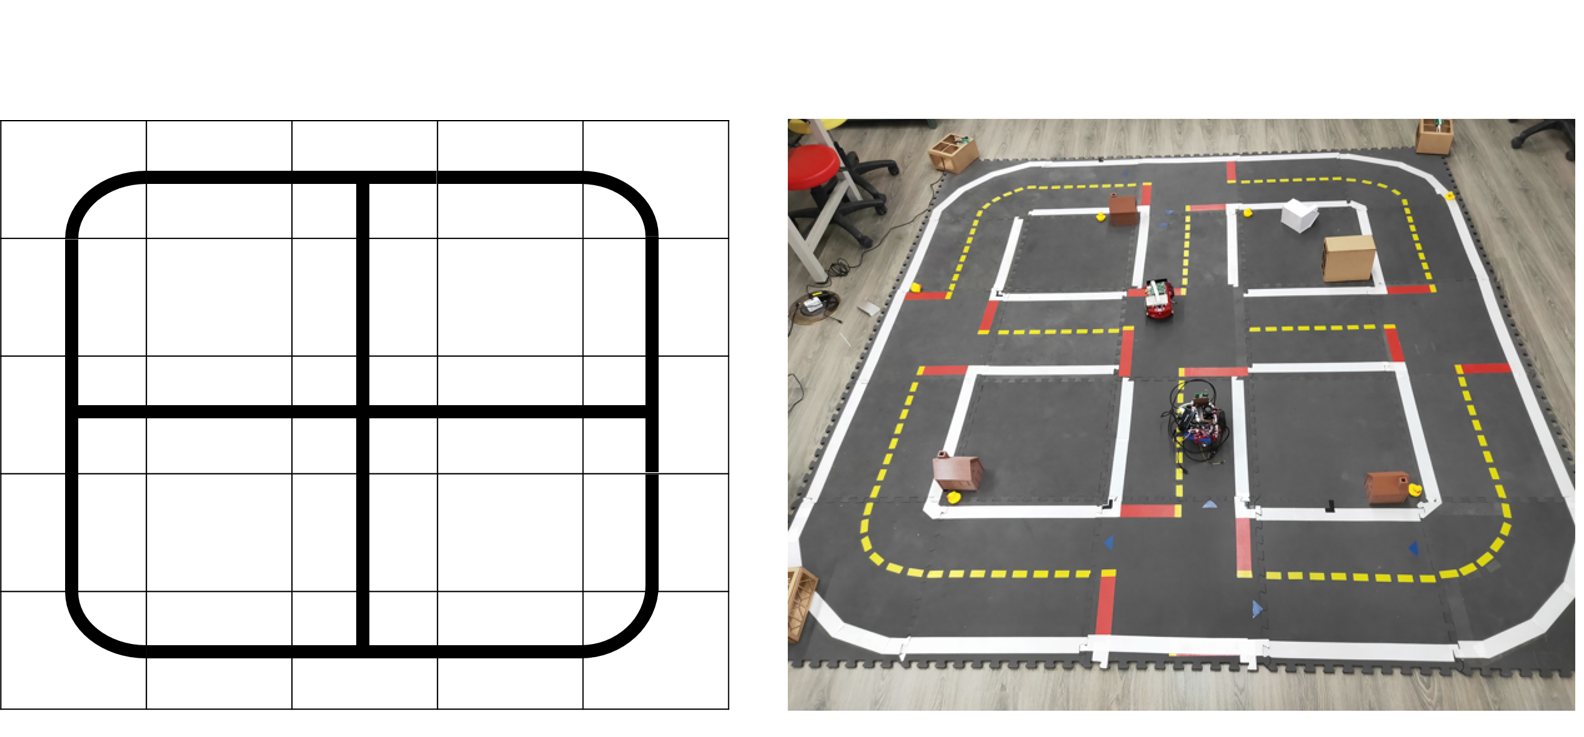
\includegraphics[width=\columnwidth]{images/field.png}
        \caption{模擬城市場地設計}
 \label{figure:field}
\end{figure}

\subsection{Localization}
我們採用Ultra-wideband作為取得定位資訊的裝置,使用pypozyx函式庫,利用UWB Anchor的訊號強度與TWR(Two Way Ranging)定位技術(圖\ref{figure:uwb_tech})同時利用三個以上的Anchor裝置就能定位出2D座標,同時利用四個以上能定位3D座標。同時UWB裝置上也搭載IMU感測器,能夠知道UWB裝置的方向。結合位置與方向這兩樣資訊我們能夠得出固定在車上的TAG三維姿態(Pose)。

\begin{figure}[h]
  \centering
    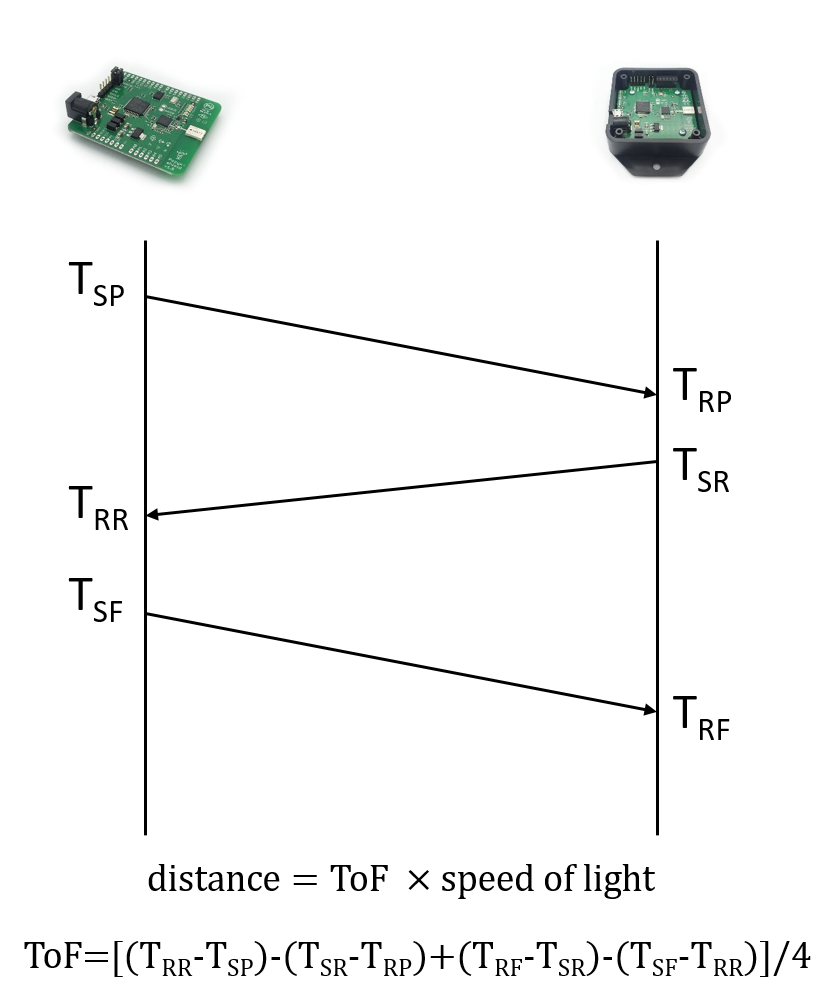
\includegraphics[width=\columnwidth]{images/uwb_tech.png}
        \caption{UWB Localization TWR technique}
 \label{figure:uwb_tech}
\end{figure}

\subsection{Vision}
在核災中,我們必須辨識出該城市內之物品,找出可能的目標物品以及生還者。
由於此次人本專題我們使用了Duckietown城市模擬核災發生並作為驗證場地,所以重新組裝了一台Super Duckiebot。
在視覺部份因考量到車體大小,故選擇使用體積較小的Jetson Nano處理相關視覺運算,同時也使用運算量較小的MobileNet-SSD Model,在影像辨識部份利用RGB資訊進行Training,精準度、輕巧度及靈敏度是Artifact search相當重要的指標,控制訓練後Model的大小將其放置於較輕巧的Jetson Nano上運行,並且考量到幀數(FPS)也就是一秒讀取幾張圖片進行辨識,各個環節環環相扣。

當辨識出目標物後,隨即使用Depth資訊利用投影矩陣取得目標物與相機之相對座標,結合UWB定位所取得之姿態訊息,定位出目標物之絕對位置,最後呈現於Rviz。

\begin{figure}[h]
  \centering
    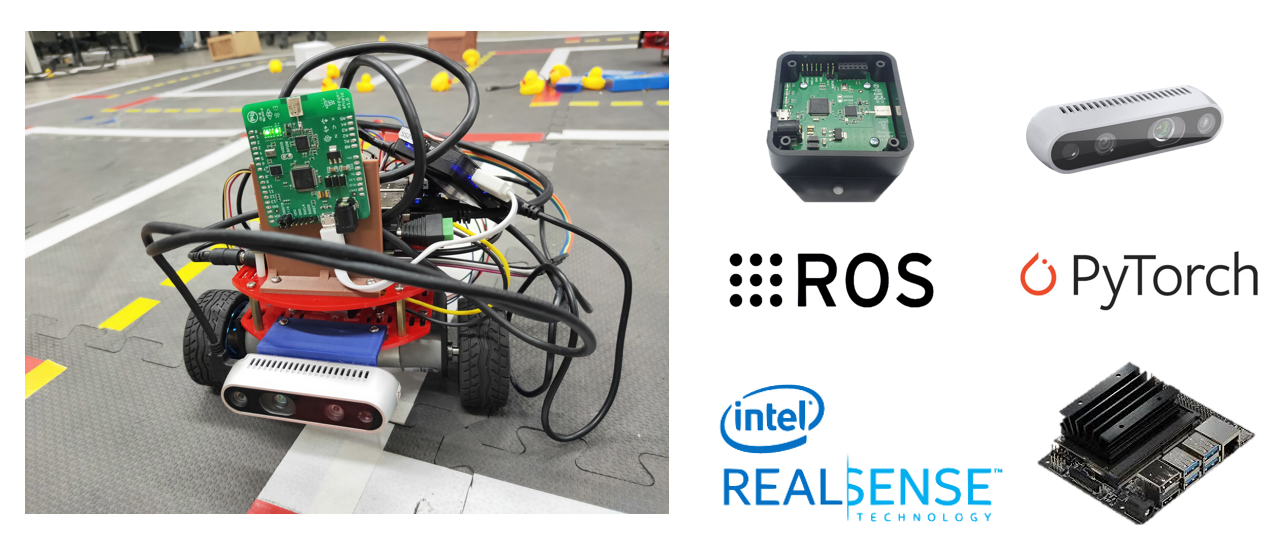
\includegraphics[width=\columnwidth]{images/car.png}
        \caption{車體設計及相關環境}
 \label{figure:car}
\end{figure}









